\subsubsection{KAlarm on KDE}
``\gls{kalarm} is a personal alarm message, command and email scheduler for \gls{linux} and \gls{unix}. \\ You can schedule alarm messages to pop up on the screen (with sound if desired), or you can schedule audio to play, commands to execute or emails to send.'' \cite{kalarm_handbook} \\

Aside from control through the graphical interface KAlarm can also be operated using the command line.

\begin{figure}[h]
\centering
\caption{\gls{kalarm} main window on KDE}
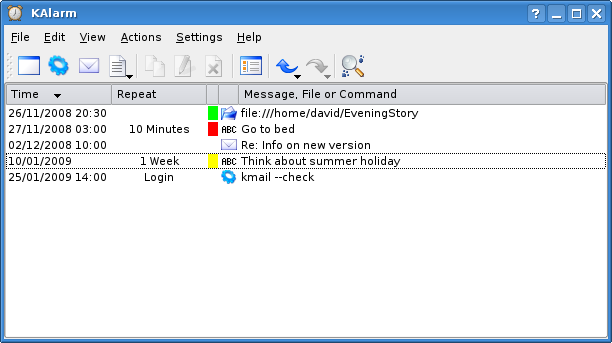
\includegraphics[width=0.7\textwidth]{kalarm.png}
\end{figure}

\subsubsection{The ClockAlarm Project}
KAlarm was officially launched in 2001. The latest update is dated 13 October 2015. Despite the recent updates, the program is aging, and is only available on Linux and UNIX platforms.\\
The goal of the mandate is to develop a new version of kAlarm, called clockAlarm. The new version is intended to replace kAlarm by offering the user the same services regardless of the platform used. The desired product therefore consists of a cross-platform program of persistent management of customizable reminders/alerts.\\
Depending on the progress of the project, it would be good to bring to the program freshness in terms of design and interaction with the user, compared to the version on KDE.